\chapter{Część programowa}

Ta część projektu odpowiada za analizę nadchodzących z wejść sygnałów i podejmowanie decyzji o wyzwoleniu zapisu na podstawie konfiguracji ustawionej przez użytkownika. 


\section{Układ próbkujący}
	Pierwszym elementem, który należało wykonać był układ próbkujący. To on odpowiedzialny jest za wyzwolenie zapisu próbek do pamięci i jego kontrolę. Z każdym narastającym zboczem zegara, kiedy sygnał \emph{CE} jest wysoki, następuje sprawdzanie, czy sygnał wejściowy się zmienił w określony sposób. Rodzaje śledzonych zmian zależą od wejścia \emph{TRIG\_KIND}. Wejście to dzieli się na 16 2-bitowych wektorów, których wartości przekładają się na zdarzenie wyzwalające zapis danych. Dla każdego z 16 wejść są to kolejno:
	
	\begin{itemize}
		\item "00" - brak wzoru wyzwalającego
		\item "01" - wyzwolenie zboczem narastającym
		\item "10" - wyzwalanie zboczem opadającym
		\item "11" - wyzwalanie zarówno zboczem narastającym jak i opadającym
	\end{itemize}
	
Początkowo jak i po resecie, wyjście \emph{WREN} jest w stanie wysokim, aby móc natychmiastowo zapisać pierwszą próbkę tuz po wyzwoleniu. Stan sygnału \emph{WREN} jest sterowany tak, aby zapisywać wartości od pierwszej próbki aż do ostatniej. Sygnał \emph{Q} odświeża się po uzyskaniu nowej próbki i zmianie adresu zapisu (sygnał \emph{ADDRQ}) na odpowiedni.
Po zresetowaniu, układ przełącza się w tryb nasłuchiwania sygnału wejściowego w oczekiwaniu na wzór wyzwalający.
Schemat blokowy modułu przedstawiono na rysunku \ref{sampler_block_diagram}

\begin{figure}[H]
	\centering
	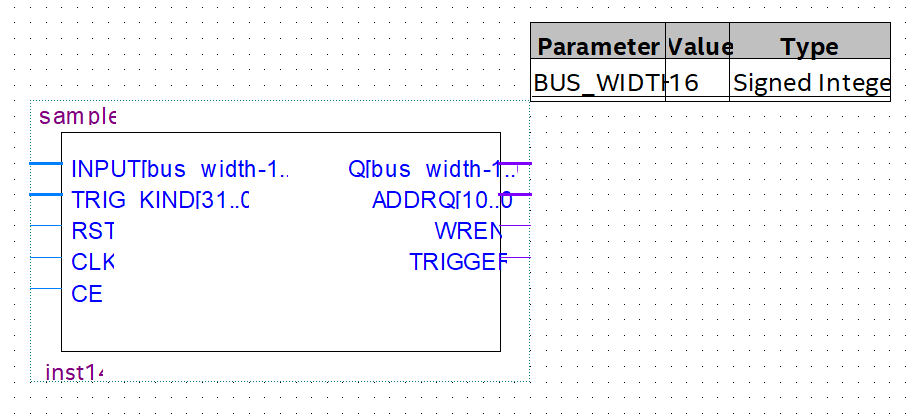
\includegraphics[width = 0.4 \paperwidth]{images/sampler_block_diagram.png}
	\caption{Blok układu próbkującego}
	\label{sampler_block_diagram}
\end{figure}
	
	
\section{Pamięć RAM}
	Pamięć RAM jest zaimplementowanym przez producenta układu FPGA modułem dwuportowej pamięci BRAM. Latencja operacji odczytu to jeden cykl zegarowy, gdyż zrezygnowano z przerzutników na wyjściu pamięci.
\section{Preskaler}
	Układ ten w odróżnieniu od pozostałych, zmienia stan sygnału wejściowego na opadającym zboczu zegara. Przekłada się to na wysoce ułatwioną analizę poprawności pracy modułów.
	Jest to preskaler, który steruje wyjściem \emph{CE} w taki sposób, aby miało wysoki stan po doliczeniu do liczby, która znajduje się na jego wejściu o nazwie \emph{PRESCALING\_FACTOR} lub od parametru podanego podczas jego deklaracji. W tym projekcie preskaler ustawiany parametrem mógłby być składowym elementem układu debouncera, jednak zdecydowano o jego braku ze względu na sprzętowy debouncing.
	Jedna instancja tego modułu w wersji nastawnej pełni rolę dzielnika częstotliwości próbkowania.
	Schemat blokowy modułu znajduje się na rysunku \ref{prescaler_block_diagram}.
	
	\begin{figure}[H]
	\centering
	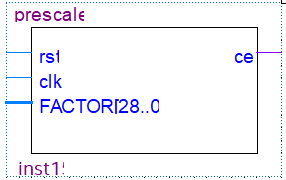
\includegraphics[width = 0.3 \paperwidth]{images/prescaler_block_diagram.png}
	\caption{Blok preskalera}
	\label{prescaler_block_diagram}
	\end{figure}
\section{Kontroler sygnałów synchronizacji obrazu} 
Moduł kontrolera sygnałów sygnalizacji obrazu jest elementem wskazującym współrzędne piksela aktualnie rysowanego na ekranie (\emph{X} oraz \emph{Y}) oraz steruje sygnałami synchronizacji pionowej i poziomej. (\emph{V\_SYNC} i \emph{H\_SYNC})
Moduł posiada również wyjście sygnału \emph{DISP\_EN} służące do łatwego określenia tego, czy obecnie rysowany jest piksel widocznej, czy ukrytej części obrazu. (ang. \emph{porch})
Blok modułu pokazano na rysunku \ref{VGA_controller_block_diagram}

\begin{figure}[H]
	\centering
	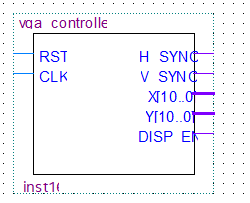
\includegraphics[width = 0.3 \paperwidth]{images/VGA_controller_block_diagram.png}
	\caption{Blok kontrolera sygnałów synchronizacji obrazu}
	\label{VGA_controller_block_diagram}
\end{figure}



\section{Generator obrazu}
Za ten blok odpowiedzialna była pani Magda, jednak nie został on ukończony. Nie mamy dostępu do postępów pracy nad tą częścią.

\section{Podsumowanie}
Symulacje wszystkich ukończonych modułów odbyły się z sukcesem, dodatkowo przetestowano ich współgranie, obecnie bez modułu rysującego obraz.
Warstwa \emph{top} projektu została pokazana na rysunku \ref{top_block_diagram}.

\begin{figure}[H]
	\centering
	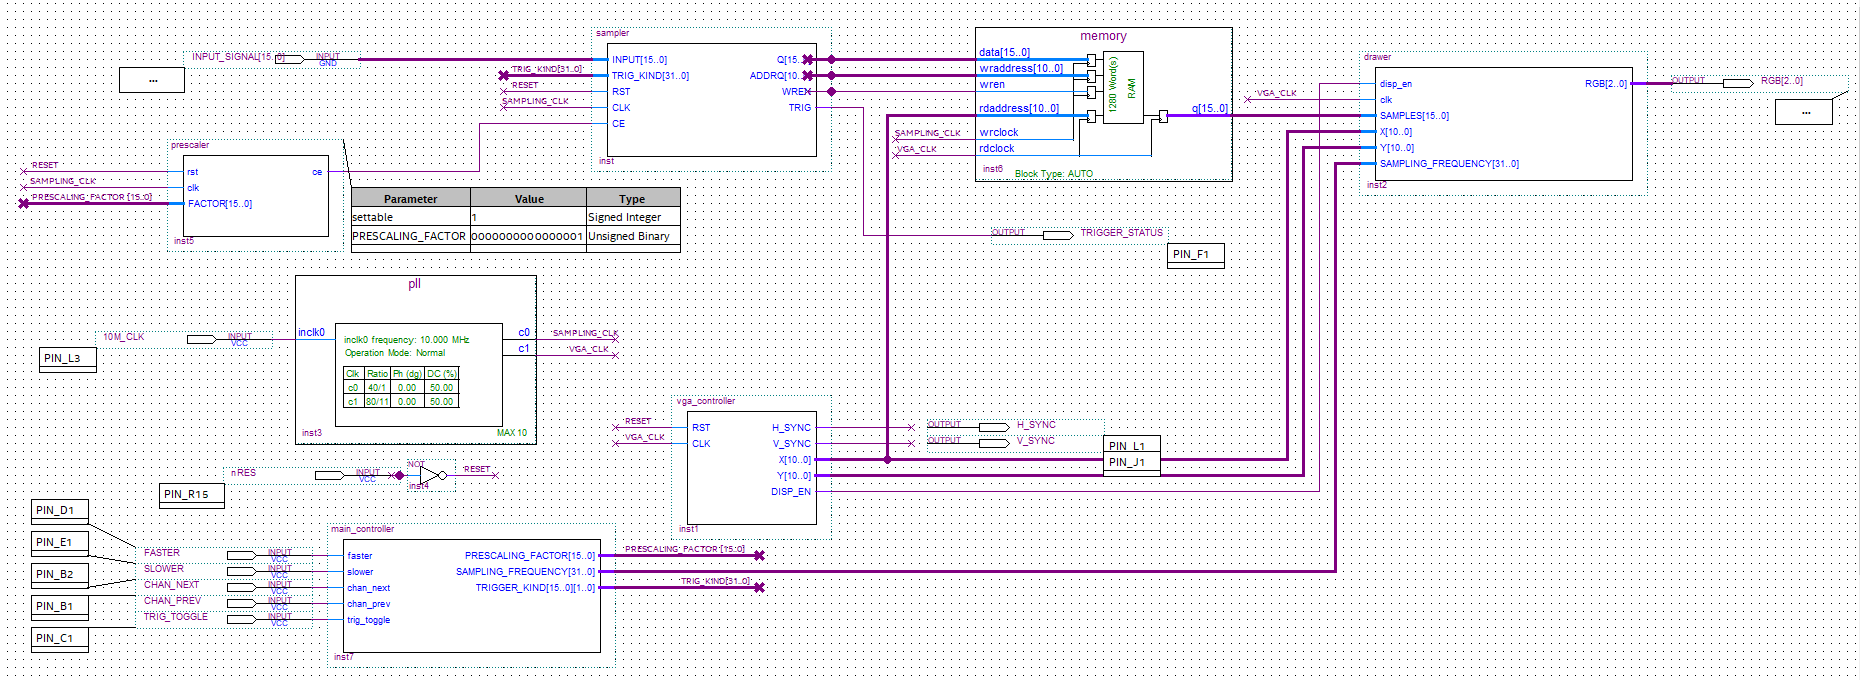
\includegraphics[width = 0.75\paperwidth]{images/top_block_diagram.png}
	\caption{Schemat blokowy warstwy \emph{top}}
	\label{top_block_diagram}
\end{figure}

